\input{"preamble.tex"}

\addbibresource{FourManifolds.bib}

\let\Begin\begin
\let\End\end
\newcommand\wrapenv[1]{#1}

\makeatletter
\def\ScaleWidthIfNeeded{%
 \ifdim\Gin@nat@width>\linewidth
    \linewidth
  \else
    \Gin@nat@width
  \fi
}
\def\ScaleHeightIfNeeded{%
  \ifdim\Gin@nat@height>0.9\textheight
    0.9\textheight
  \else
    \Gin@nat@width
  \fi
}
\makeatother

\setkeys{Gin}{width=\ScaleWidthIfNeeded,height=\ScaleHeightIfNeeded,keepaspectratio}%

\title{
\textbf{
    4-Manifolds
  }
    \\ {\normalsize Lectures by Philip Engel. University of Georgia,
Spring 2020} \\
  }







\begin{document}

\date{}
\author{D. Zack Garza}
\maketitle
\begin{flushleft}
\textit{D. Zack Garza} \\
\textit{University of Georgia} \\
  \textit{\href{mailto: dzackgarza@gmail.com}{dzackgarza@gmail.com}} \\
{\tiny \textit{Last updated:} 2021-01-16 }
\end{flushleft}


\newpage

% Note: addsec only in KomaScript
\addsec{Table of Contents}
\tableofcontents
\newpage

\def\contradiction
{
\tikz[baseline, x=0.2em, y=0.2em, line width=0.04em]
\draw (0,0) -- ({4*cos(45)},{4*sin(45)})
    (-1,1) -- ({-1 + 4*cos(45)},{1 + 4*sin(45)})
    (-1,3) -- ({-1 + 4*cos(315)},{3 + 4*sin(315)})
    (0,4) -- ({0 + 4*cos(315)},{4 + 4*sin(315)});
}

\hypertarget{tuesday-january-12}{%
\section{Tuesday, January 12}\label{tuesday-january-12}}

\hypertarget{background}{%
\subsection{Background}\label{background}}

From Phil's email:

There are very few references in the notes, and I'll try to update them
to include more as we go. Personally, I found the following online
references particularly useful:

\begin{itemize}
\item
  Dietmar Salamon: Spin Geometry and Seiberg-Witten Invariants
  \autocite{Dietmar99}
\item
  Richard Mandelbaum: Four-dimensional Topology: An Introduction
  \autocite{Mandelbaum1980}

  \begin{itemize}
  \tightlist
  \item
    This book has a nice introduction to surgery aspects of
    four-manifolds, but as a warning: It was published right before
    Freedman's famous theorem. For instance, the existence of an exotic
    R\^{}4 was not known. This actually makes it quite useful, as a
    summary of what was known before, and provides the historical
    context in which Freedman's theorem was proven.
  \end{itemize}
\item
  Danny Calegari: Notes on 4-Manifolds \autocite{Calegari}
\item
  Yuli Rudyak: Piecewise Linear Structures on Topological Manifolds
  \autocite{Rudyak}
\item
  Akhil Mathew: The Dirac Operator \autocite{Matthew}
\item
  Tom Weston: An Introduction to Cobordism Theory \autocite{Weston}

  A wide variety of lecture notes on the Atiyah-Singer index theorem,
  which are available online.
\end{itemize}

\hypertarget{introduction}{%
\subsection{Introduction}\label{introduction}}

\begin{definition}[Topological Manifold]

Recall that a \textbf{topological manifold} (or \(C^0\) manifold) \(X\)
is a Hausdorff topological space \emph{locally homeomorphic} to
\({\mathbb{R}}^n\) with a countable topological base, so we have charts
\(\phi_u: U\to {\mathbb{R}}^n\) which are homeomorphisms from open sets
covering \(X\).

\end{definition}

\begin{example}[The circle]

\(S^1\) is covered by two charts homeomorphic to intervals:

\begin{figure}
\centering
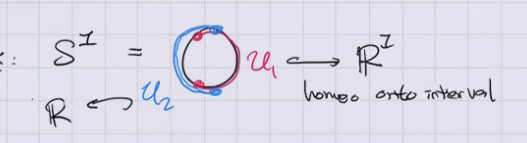
\includegraphics{figures/image_2021-01-13-14-02-19.png}
\caption{image\_2021-01-13-14-02-19}
\end{figure}

\end{example}

\begin{remark}

Maps that are merely continuous are poorly behaved, so we may want to
impose extra structure. This can be done by imposing restrictions on the
transition functions, defined as
\begin{align*}
t_{uv} \coloneqq\varphi_V \to \varphi_U ^{-1} : \varphi_U(U \cap V) \to \varphi_V(U \cap V)
.\end{align*}

\end{remark}

\begin{definition}[Restricted Structures on Manifolds]

\envlist

\begin{itemize}
\item
  We say \(X\) is a \textbf{PL manifold} if and only if \(t_{UV}\) are
  piecewise-linear. Note that an invertible PL map has a PL inverse.
\item
  We say \(X\) is a \textbf{\(C^k\) manifold} if they are \(k\) times
  continuously differentiable, and \textbf{smooth} if infinitely
  differentiable.
\item
  We say \(X\) is \textbf{real-analytic} if they are locally given by
  convergent power series.
\item
  We say \(X\) is \textbf{complex-analytic} if under the identification
  \({\mathbb{R}}^n \cong {\mathbb{C}}^{n/2}\) if they are holomorphic,
  i.e.~the differential of \(t_{UV}\) is complex linear.
\item
  We say \(X\) is a \textbf{projective variety} if it is the vanishing
  locus of homogeneous polynomials on \({\mathbb{CP}}^N\).
\end{itemize}

\end{definition}

\begin{remark}

Is this a strictly increasing hierarchy? It's not clear e.g.~that every
\(C^k\) manifold is PL.

\end{remark}

\begin{question}

Consider \({\mathbb{R}}^n\) as a topological manifold: are any two
smooth structures on \({\mathbb{R}}^n\) diffeomorphic?

\end{question}

\begin{remark}

Fix a copy of \({\mathbb{R}}\) and form a single chart
\({\mathbb{R}}\xrightarrow{\operatorname{id}} {\mathbb{R}}\). There is
only a single transition function, the identity, which is smooth. But
consider
\begin{align*}
X &\to {\mathbb{R}}\\
t &\mapsto t^3
.\end{align*}
This is also a smooth structure on \(X\), since the transition function
is the identity. This yields a different smooth structure, since these
two charts don't like in the same maximal atlas. Otherwise there would
be a transition function of the form \(t_{VU}: t\mapsto t^{1/3}\), which
is not smooth at zero. However, the map
\begin{align*}
X &\to X \\
t &\mapsto t^3
.\end{align*}
defines a diffeomorphism between the two smooth structures.

\end{remark}

\begin{claim}

\({\mathbb{R}}\) admits a unique smooth structure.

\end{claim}

\begin{proof}[sketch]

Let \(\tilde {\mathbb{R}}\) be some exotic \({\mathbb{R}}\), i.e.~a
smooth manifold homeomorphic to \({\mathbb{R}}\). Cover this by
coordinate charts to the standard \({\mathbb{R}}\):

\begin{figure}
\centering
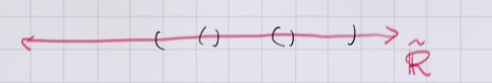
\includegraphics{figures/image_2021-01-13-14-22-18.png}
\caption{image\_2021-01-13-14-22-18}
\end{figure}

\begin{fact}

There exists a cover which is \emph{locally finite} and supports a
\emph{partition of unity}: a collection of smooth functions
\(f_i: U_i \to {\mathbb{R}}\) with \(f_i \geq 0\) and
\({\operatorname{supp}}f \subseteq U_i\) such that \(\sum f_i = 1\)
(\emph{i.e., bump functions}). It is also a purely topological fact that
\(\tilde {\mathbb{R}}\) is orientable.

\end{fact}

So we have bump functions:

\begin{figure}
\centering
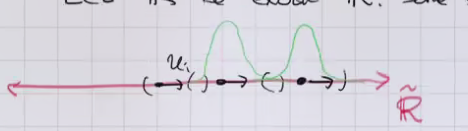
\includegraphics{figures/image_2021-01-13-14-25-30.png}
\caption{image\_2021-01-13-14-25-30}
\end{figure}

Take a smooth vector field \(V_i\) on \(U_i\) everywhere aligning with
the orientation. Then \(\sum f_i V_i\) is a smooth nowhere vector field
on \(X\) that is nowhere zero in the direction of the orientation.
Taking the associated flow
\begin{align*}
{\mathbb{R}}&\to \tilde {\mathbb{R}}\\
t &\mapsto \varphi(t)
.\end{align*}
such that \(\varphi'(t) = V(\varphi(t))\). Then \(\varphi\) is a smooth
map that defines a diffeomorphism. This follows from the fact that the
vector field is everywhere positive.

\begin{slogan}

To understand smooth structures on \(X\), we should try to solve
differential equations on \(X\).

\end{slogan}

\end{proof}

\begin{remark}

Note that here we used the existence of a global frame, i.e.~a
trivialization of the tangent bundle, so this doesn't quite work for
e.g.~\(S^2\).

\end{remark}

\begin{question}

What is the difference between all of the above structures? Are there
obstructions to admitting any particular one?

\end{question}

\begin{answer}

\envlist

\begin{enumerate}
\def\labelenumi{\arabic{enumi}.}
\item
  (Munkres) Every \(C^1\) structure gives a unique \(C^k\) and
  \(C^ \infty\) structure.\footnote{Note that this doesn't start at
    \(C^0\), so topological manifolds are genuinely different! There
    exist topological manifolds with no smooth structure.}
\item
  (Grauert) Every \(C^ \infty\) structure gives a unique real-analytic
  structure.
\item
  Every PL manifold admits a smooth structure in \(\dim X \leq 7\), and
  it's unique in \(\dim X\leq 6\), and above these dimensions there
  exists PL manifolds with no smooth structure.
\item
  (Kirby--Siebenmann) Let \(X\) be a topological manifold of
  \(\dim X\geq 5\), then there exists a cohomology class
  \(\operatorname{ks}(X) \in H^4(X; {\mathbb{Z}}/2{\mathbb{Z}})\) which
  is 0 if and only if \(X\) admits a PL structure. Moreover, if
  \(\operatorname{ks}(X) = 0\), then (up to concordance) the set of PL
  structures is given by \(H^3(X; {\mathbb{Z}}/2{\mathbb{Z}})\).
\item
  (Moise) Every topological manifold in \(\dim X\leq 3\) admits a unique
  smooth structure.
\item
  (Smale et al.): In \(\dim X\geq 5\), the number of smooth structures
  on a topological manifold \(X\) is finite. In particular,
  \({\mathbb{R}}^n\) for \(n \neq 4\) has a unique smooth structure. So
  dimension 4 is interesting!
\item
  (Taubes) \({\mathbb{R}}^4\) admits uncountably many non-diffeomorphic
  smooth structures.
\item
  A compact oriented smooth surface \(\Sigma\), the space of
  complex-analytic structures is a complex orbifold \footnote{Locally
    admits a chart to \({\mathbb{C}}^n/ \Gamma\) for \(\Gamma\) a finite
    group.} of dimension \(3g-2\) where \(g\) is the genus of
  \(\Sigma\), up to biholomorphism (i.e.~\emph{moduli}).
\end{enumerate}

\end{answer}

\begin{remark}

Kervaire-Milnor: \(S^7\) admits 28 smooth structures, which form a
group.

\end{remark}

\hypertarget{friday-january-15}{%
\section{Friday, January 15}\label{friday-january-15}}

\begin{remark}

Let
\begin{align*}
V &\coloneqq\left\{{a^2 + b^2 + c^2 + d^3 + e^{6k-1} = 0}\right\} \subseteq {\mathbb{C}}^5 \\
S_\varepsilon&\coloneqq\left\{{ {\left\lvert {a} \right\rvert}^2 + {\left\lvert {b} \right\rvert}^2 + {\left\lvert {c} \right\rvert}^2 + {\left\lvert {d} \right\rvert}^2 + {\left\lvert {e} \right\rvert}^2}\right\}
.\end{align*}
Then \(V_k \cap S_\varepsilon\cong S^7\) is a homeomorphism, and taking
\(k=1,2,\cdots, 28\) yields the 28 smooth structures on \(S^7\). Note
that \(V_k\) is the cone over \(V_k \cap S_\varepsilon\).

\begin{figure}
\centering
\resizebox{\columnwidth}{!}{%
\begin{tikzpicture}
\node (node_one) at (0,0) { \import{/home/zack/SparkleShare/github.com/Notes/Class_Notes/2021/Spring/FourManifolds/sections/figures/}{2021-01-15_13-54.pdf_tex} };
\end{tikzpicture}
}
\end{figure}

\begin{quote}
? Admits a smooth structure, and
\(\mkern 1.5mu\overline{\mkern-1.5muV\mkern-1.5mu}\mkern 1.5mu_k \subseteq {\mathbb{CP}}^5\)
admits no smooth structure.
\end{quote}

\end{remark}

\begin{question}

Is every triangulable manifold PL, i.e.~homeomorphic to a simplicial
complex?

\end{question}

\begin{answer}

No! Given a simplicial complex, there is a notion of the
\textbf{combinatorial link} of a vertex.

\begin{figure}
\centering
\resizebox{\columnwidth}{!}{%
\begin{tikzpicture}
\node (node_one) at (0,0) {
\import{/home/zack/SparkleShare/github.com/Notes/Class_Notes/2021/Spring/FourManifolds/sections/figures/}{2021-01-15_13-57.pdf_tex} };
\end{tikzpicture}
}
\end{figure}

It turns out that there exist simplicial manifolds such that the link is
not homeomorphic to a sphere, whereas every PL manifold admits a ``PL
triangulation'' where the links are spheres.

\end{answer}

\begin{remark}

What's special in dimension 4? Recall the \textbf{Kirby-Siebenmann}
invariant \(\operatorname{ks}(x) \in H^4(X; {\mathbb{Z}}_2)\) for \(X\)
a topological manifold where \(\operatorname{ks}(X) = 0 \iff X\) admits
a PL structure, with the caveat that \(\dim X \geq 5\). We can use this
to cook up an invariant of 4-manifolds.

\end{remark}

\begin{definition}[Kirby-Siebenmann Invariant of a 4-manifold]

Let \(X\) be a topological 4-manifold, then
\begin{align*}
\operatorname{ks}(X) \coloneqq\operatorname{ks}(X \times{\mathbb{R}})
.\end{align*}

\end{definition}

\begin{remark}

Recall that in \(\dim X\geq 7\), every PL manifold admits a smooth
structure, and we can note that
\begin{align*}
H^4(X; {\mathbb{Z}}_2) = H^4(X \times{\mathbb{R}}; {\mathbb{Z}}_2) = {\mathbb{Z}}_2,
.\end{align*}
since every oriented 4-manifold admits a fundamental class. Thus
\begin{align*}
\operatorname{ks}(X) = 
\begin{cases}
0 & X \times{\mathbb{R}}\text{ admits a PL and smooth structure} 
\\
1 & X \times{\mathbb{R}}\text{ admits no PL or smooth structures }.
\end{cases}
\end{align*}

\end{remark}

\begin{remark}

\(\operatorname{ks}(X) \neq 0\) implies that \(X\) has no smooth
structure, since \(X \times{\mathbb{R}}\) doesn't. Note that it was not
known if this invariant was nonzero for a while!

\end{remark}

\begin{remark}

Note that \(H^2(X; {\mathbb{Z}})\) admits a symmetric bilinear form
\(Q_X\) defined by
\begin{align*}
{\left\langle { \alpha},~{ \beta} \right\rangle} \mapsto \int_X \alpha\wedge \beta = \alpha \smile\beta([X]) \in {\mathbb{Z}}
.\end{align*}
where \([X]\) is the fundamental class.

\end{remark}

\hypertarget{main-theorems-for-the-course}{%
\section{Main Theorems for the
Course}\label{main-theorems-for-the-course}}

Proving the following theorems is the main goal of this course.

\begin{theorem}[Freedman]

If \(X, Y\) are compact oriented topological 4-manifolds, then
\(X\cong Y\) are homeomorphic if and only if
\(\operatorname{ks}(X) = \operatorname{ks}(Y)\) and \(Q_X \cong Q_Y\)
are isometric, i.e.~there exists an isometry
\begin{align*}
\varphi: H^2(X; {\mathbb{Z}}) \to H^2(Y; {\mathbb{Z}})
.\end{align*}
that preserves the two bilinear forms in the sense that
\({\left\langle {\varphi \alpha},~{ \varphi \beta} \right\rangle} = {\left\langle { \alpha},~{ \beta} \right\rangle}\).

Conversely, every \textbf{unimodular} bilinear form appears as
\(H^2(X; {\mathbb{Z}})\) for some \(X\), i.e.~the pairing induces a map
\begin{align*}
H^2(X; {\mathbb{Z}}) &\to H^2(X; {\mathbb{Z}})^\vee\\
\alpha \mapsto {\left\langle { \alpha },~{ {\,\cdot\,}} \right\rangle}
.\end{align*}
which is an isomorphism. This is essentially a classification of
simply-connected 4-manifolds.

\end{theorem}

\begin{remark}

Note that preservation of a bilinear form is a stand-in for ``being an
element of the orthogonal group'', where we only have a lattice instead
of a full vector space.

\end{remark}

\begin{remark}

There is a map
\(H^2(X; {\mathbb{Z}}) \xrightarrow{PD} H_2(X; {\mathbb{Z}})\) from
Poincaré , where we can think of elements in the latter as closed
surfaces \([\Sigma]\), and
\begin{align*}
{\left\langle { \Sigma_1 },~{ \Sigma_2 } \right\rangle} = \text{signed number of intersections points of } \Sigma_1 \pitchfork\Sigma_2
.\end{align*}
Note that Freedman's theorem is only about homeomorphism, and is not
true smoothly. This gives a way to show that two 4-manifolds are
homeomorphic, but this is hard to prove! So we'll black-box this, and
focus on ways to show that two \emph{smooth} 4-manifolds are \emph{not}
diffeomorphic, since we want homeomorphic but non-diffeomorphic
manifolds.

\end{remark}

\begin{definition}[Signature]

The \textbf{signature} of a topological 4- manifold is the signature of
\(Q_X\), where we note that \(Q_X\) is a symmetric nondegenerate
bilinear form on \(H^2(X; {\mathbb{R}})\) and for some \(a, b\)
\begin{align*}
(H^2(X; {\mathbb{R}}), Q_x) \xrightarrow{\text{isometric}} {\mathbb{R}}^{a, b}
.\end{align*}
where \(a\) is the number of \(+1\)s appearing in the matrix and \(b\)
is the number of \(-1\)s. This is \({\mathbb{R}}^{ab}\) where
\(e_i^2 = 1, i=1\cdots a\) and \(e_i^2 = -1, i=a+1, \cdots b\), and is
thus equipped with a specific bilinear form corresponding to the Gram
matrix of this basis.
\begin{align*}
\begin{bmatrix}
1 & 0 & 0 & 0 & 0
\\
0 & 1 & 0 & 0 & 0
\\
0 & 0 & \ddots & 0 & 0
\\
0 & 0 & 0 & -1 & 0
\\
0 & 0 & 0 & 0 & -1
\end{bmatrix}
= I_{a\times a} \oplus -I_{b \times b}
.\end{align*}
Then the signature is \(a-b\), the dimension of the positive-definite
space minus the dimension of the negative-definite space.

\end{definition}

\begin{theorem}[Rokhlin's Theorem]

Suppose
\({\left\langle { \alpha},~{\alpha} \right\rangle} \in 2{\mathbb{Z}}\)
and \(\alpha\in H^2(X; {\mathbb{Z}})\) and \(X\) a simply connected
\textbf{smooth} 4-manifold. Then 16 divides \(\operatorname{sig}(X)\).

\end{theorem}

\begin{remark}

Note that Freedman's theorem implies that there exists topological
4-manifolds with no smooth structure.

\end{remark}

\begin{theorem}[Donaldson]

Let \(X\) be a smooth simply-connected 4-manifold. If \(a=0\) or
\(b=0\), then \(Q_X\) is diagonalizable and there exists an orthonormal
basis of \(H^2(X; {\mathbb{Z}})\).

\end{theorem}

\begin{remark}

This comes from Gram-Schmidt, and restricts what types of intersection
forms can occur.

\end{remark}

\hypertarget{warm-up-mathbbr2-has-a-unique-smooth-structure}{%
\subsection{\texorpdfstring{Warm Up: \({\mathbb{R}}^2\) Has a Unique
Smooth
Structure}{Warm Up: \{\textbackslash mathbb\{R\}\}\^{}2 Has a Unique Smooth Structure}}\label{warm-up-mathbbr2-has-a-unique-smooth-structure}}

\begin{remark}

Last time we showed \({\mathbb{R}}^1\) had a unique smooth structure, so
now we'll do this for \({\mathbb{R}}^2\). The strategy of solving a
differential equation, we'll now sketch the proof.

\end{remark}

\begin{definition}[Riemannian Metrics]

A \textbf{Riemannian metric} \(g\in \operatorname{Sym}^2 T^*X\) for
\(X\) a smooth manifold is a metric on every \(T_p X\) given by
\begin{align*}
g_p: T_pX \times T_p X &\to {\mathbb{R}}\\
g(v, v) \geq 0, g(v,v) = 0 \iff v=0
.\end{align*}

\end{definition}

\begin{definition}[Almost complex structure]

An \textbf{almost complex structure} is a
\(J\in \mathop{\mathrm{End}}(TX)\) such that
\(J^2 = -\operatorname{id}\).

\end{definition}

\begin{remark}

Let \(e\in T_p X\) and \(e\neq 0\), then if \(X\) is a surface then
\(\left\{{e, Je}\right\}\) is a basis of \(T_p X\).

\begin{figure}
\centering
\resizebox{\columnwidth}{!}{%
\begin{tikzpicture}
\node (node_one) at (0,0) { \import{/home/zack/SparkleShare/github.com/Notes/Class_Notes/2021/Spring/FourManifolds/sections/figures/}{2021-01-15_14-33.pdf_tex} };
\end{tikzpicture}
}
\end{figure}

This is a basis because if \(Je\) and \(e\) are parallel, then ??? In
particular, \(J_p\) is determined by a point in
\({\mathbb{R}}^2\setminus\left\{{\text{the }x{\hbox{-}}\text{axis}}\right\}\)

\end{remark}

\hypertarget{sketch-of-proof}{%
\subsubsection{Sketch of Proof}\label{sketch-of-proof}}

Let \(\tilde {\mathbb{R}}^2\) be an exotic \({\mathbb{R}}^2\).

\hypertarget{step-1}{%
\paragraph{Step 1}\label{step-1}}

Choose a metric on \(\tilde {\mathbb{R}}^2\) \(g \coloneqq\sum f_I g_i\)
with \(g_i\) metrics on coordinate charts \(U_i\) and \(f_i\) a
partition of unity.

\hypertarget{step-2}{%
\paragraph{Step 2}\label{step-2}}

Find an almost complex structure on \(\tilde {\mathbb{R}}^2\). Choosing
an orientation of \(\tilde {\mathbb{R}}^2\), \(g\) defines a unique
almost complex structure
\(J_p e \coloneqq f\in T_p \tilde {\mathbb{R}}^2\) such that

\begin{itemize}
\tightlist
\item
  \(g(e, e) = g(f, f)\)
\item
  \(g(e, f) = 0\).
\item
  \(\left\{{e, f}\right\}\) is an oriented basis of
  \(T_p \tilde {\mathbb{R}}^2\)
\end{itemize}

This is because after choosing \(e\), there are two orthogonal vectors,
but only one choice yields an \emph{oriented} basis.

\begin{figure}
\centering
\resizebox{\columnwidth}{!}{%
\begin{tikzpicture}
\node (node_one) at (0,0) {
  \import{/home/zack/SparkleShare/github.com/Notes/Class_Notes/2021/Spring/FourManifolds/sections/figures/}{2021-01-15_14-39.pdf_tex}
  };
\end{tikzpicture}
}
\end{figure}

\hypertarget{step-3}{%
\paragraph{Step 3}\label{step-3}}

We then apply a theorem:

\begin{theorem}[?]

Any almost complex structure on a surface comes from a complex
structure, in the sense that there exist charts
\(\varphi_i: U_i \to {\mathbb{C}}\) such that \(J\) is multiplication by
\(i\).

\end{theorem}

So \(d \varphi(J \cdot e) = i \cdot d \varphi_i (e)\), and
\((\tilde {\mathbb{R}}^2, J)\) is a complex manifold. Since it's simply
connected, the Riemann Mapping Theorem shows that it's biholomorphic to
\({\mathbb{D}}\) or \({\mathbb{C}}\), both of which are diffeomorphic to
\({\mathbb{R}}^2\).

\begin{quote}
See the Newlander-Nirenberg theorem, a result in complex geometry.
\end{quote}


\printbibliography[title=Bibliography]


\end{document}
